\chapter{The atlas as a posterior map}\label{ch:atlas}

\section{What an atlas is for}

The atlas is the set of templates the chain separates a specimen into, and the reference on which each cell's identity loci are
chosen. Every reading passes through it twice. An error in the atlas is therefore an error in every reading, and the atlas has to be
built with the same care as the sky model a CMB analysis subtracts.

\section{What the first atlas taught}

The first atlas held 114 cells at 483,092 loci, with a mean and posterior standard deviation per cell per locus. It was assembled from
other groups' reference tables, most of them marker panels of a few hundred to a few thousand CpGs, and each locus was fitted
independently. Seventy-two of its cells fell into eleven \emph{coverage families} that shared an exact count of defined loci, one dataset
each: 252, 333, 2,464, 2,543, 6,105 and so on. A cell measured at 252 loci carried the grand mean of all cells at every other locus.

Every one of the following was traced to that construction, and none to the physics:
\begin{itemize}
\item a 252-locus erythroblast profile absorbing mass from every specimen, because a flat profile fits anything a little;
\item twins: the same cell from two sources entered twice and solved apart;
\item a reproducible 0.067 misfit with no term to hold it;
\item foreign-cell templates defined on 1.3~\% of the array;
\item composition errors of $\pm0.035$ on CD4, CD8 and NK;
\item the sky's offset off the identity loci (Chapter~\ref{ch:sky}).
\end{itemize}
The author's summary of the lesson became a rule: \emph{I'd rather not have a cell than only have part of one.} A flat-filled cell is not
a partial cell; it is a false one.

\section{The model}

The second atlas is one hierarchical fit. For locus $i$, cell $c$ and source $s$ (one published data set on one platform),
\begin{align}
  \beta^{\mathrm{obs}}_{ics}&\sim\mathcal N\!\left(\mu_{ic}+\delta_{is},\ \sigma^2_{\mathrm{obs},s}+\sigma^2_{\mathrm{loc},i}\right)\quad\text{where measured},\\
  \mu_{ic}&=m_i+e_{ic},\qquad e_{ic}\sim\mathcal N(0,\tau^2),
\end{align}
with $m_i$ the locus's shared level and $\delta_{is}$ the source term: what one laboratory's platform and pipeline add to every cell it
measured. The inputs are the \emph{samples} behind each published table, at every locus they measured, so the model sees real donor-to-donor
spread. Nothing in it reads a patient, a specimen or a laboratory of patients; the floors are not refitted. Architecture class does not enter
the fit (author's decision, 28 September 2026). Two consequences follow by construction.
\begin{enumerate}
\item The same cell from two sources shares one $\mu_{ic}$ and differs only by $\delta$: twins become one cell.
\item Where a cell's sources never measured a locus, $\mu_{ic}$ is left \emph{blank}, not filled. The number of observations behind every value,
      $n_{\mathrm{obs}}$, is stored beside it.
\end{enumerate}

\section{Sources and the entry rule}

\begin{center}\small
\begin{tabular}{@{}lll@{}}\toprule
source & form & entered as \\\midrule
Moss 2018 (GSE122126) & raw 450K/EPIC IDATs & through the chain's own Stage~1 \\
Salas 2018, 2022 (GSE110554, GSE167998) & raw IDATs of sorted blood & through Stage~1 \\
GSE63409 & raw IDATs of sorted HSC and progenitors & through Stage~1 \\
Loyfer 2023 (GSE186458) & WGBS $\beta$ and depth at array CpGs & per-locus, $\ge10$ reads \\
Tian 2023 (GSE215353) & brain single-cell pseudobulk & pooled; flagged \\
ENCODE & WGBS of tissues and embryonic stem lines & per-locus, $\ge10$ reads \\\bottomrule
\end{tabular}
\end{center}
A cell enters only if it has at least two independent donors; every array passes intake and every sequencing sample has at least ten reads at
90~\% of loci; it is not a twin of an existing cell; and it reads 1.00 on its own profile. A cell failing any of these waits for data. The twin
test was made at the level of samples: a CpG counts as separating two cells only when every sample of one lies more than 0.20 beyond every sample of
the other. Sampling noise cannot manufacture that. By it, a kidney podocyte entry was found to be sorting impurity from tubule (no
hypomethylation at the podocyte genes \emph{NPHS1}, \emph{PODXL}, \emph{WT1}), and mixtures were removed. Seventy-four cells entered.

The author's ruling on what counts as a reference: \emph{a cell is a cell is a cell}; every sample, specimen or vial is a means to the methylome
sought. Profiles of whole tissues are therefore test specimens for the atlas, not references in it.

\section{Putting sequencing on the array scale}

The atlas sits on the chain's own array scale. Sequencing sources enter through their source terms, estimated in closed form: for each sequencing
source, a Deming regression of its per-locus cell means on the array means of the same cells, over 50,000 loci, with a bootstrap over cells. A first
cross-platform measurement on ten cell types measured both ways gave slopes of 1.03--1.09 and intercepts of $-0.04$ to $-0.07$ for every cell type:
one transfer between platforms, not a per-cell difference. \measured{} Two sources share no cell with any other and their terms cannot be measured:
the stem-line sequencing, which was later bridged by an embryonic-stem-cell array series with raw IDATs (GSE116754), and GSE63409's sorted
progenitors, which take an array offset of zero. The author's decision was to \emph{keep them in and notate the truth}: the progenitor source term
is carried with status ASSUMED and an estimated effect on $A$ of at most about 0.015, and every reading on those cells carries the flag.

\section{The fit}

A first attempt to fit the source terms jointly with every cell mean did not converge ($\hat R$ up to 4.3): a source's terms trade off against the
means of every cell only it measured. With the source terms fixed from the closed form, a test block of about 1,000 loci converged
($\hat R$ 99th percentile 1.005, effective sample size 1st percentile 753, no divergences), at 0.83~s per locus. The full fit then ran over about
814,000 loci in 700 blocks with NUTS~\cite{Hoffman2014} in NumPyro, on rented cloud machines, every finished block copied to storage as it landed.
Twenty posterior draws per cell per locus were kept. A whole-atlas gate confirmed that no two cells came out identical and that no value was filled
where a cell was unmeasured; 0.19~\% of values were flagged for per-block convergence and kept with the flag.

\section{Does the atlas tell the truth about itself?}

A posterior interval is only useful if it covers the truth at the stated rate. V5 hid 5~\% of the observations in 20 randomly chosen blocks, refitted
those blocks, and asked how often the held-out values fell inside the atlas's 90~\% predictive interval (Figure~\ref{fig:v5}). \measured

\begin{figure}[t]\centering
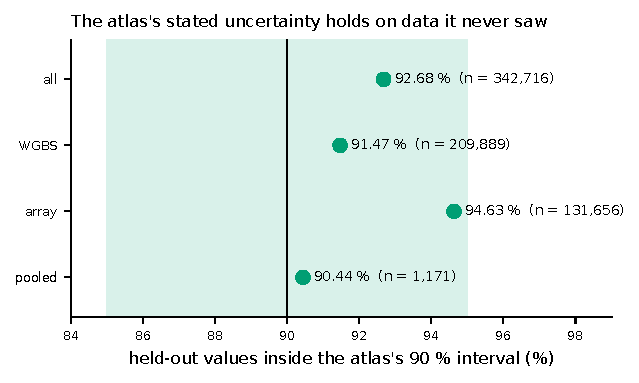
\includegraphics[width=0.75\textwidth]{figures/part4/fig_v5.pdf}
\caption{Coverage of held-out observations by the atlas v2 90~\% interval, overall and by kind of data; shaded band is the pre-registered pass range,
85--95~\%. 342,716 held-out observations in 20 blocks; every block 92.3--93.1~\%; no divergences. \measured}
\label{fig:v5}
\end{figure}

The atlas's stated uncertainty is honest and slightly conservative: 92.7~\% against a nominal 90~\%. The lowest cells were smooth muscle (82.9~\%) and
aorta and lung alveolar endothelium (about 89~\%); the highest were three bone-marrow progenitors (CMP, L-MPP, MPP) and kidney glomerular
epithelium, at 96.9--97.2~\%. Mean absolute prediction error was 0.051.

\section{What is in it}

Seventy-four cells: 22 immune, 13 cycling, 13 secretory, 12 stromal, 7 progenitor, 5 terminal, one adult stem and one pluripotent
(Figure~\ref{fig:idloci} in the next chapter). Cells the first atlas named but the second does not contain are not lost; they wait for data that meet
the entry rule. The candidate sources for the next additions, one at a time and through the same script, are the expanded purified-cell WGBS sets and the
2026 single-cell body atlas~\cite{Loyfer2023}.

\section{What this atlas does that a reference panel does not}

Methylation references in common use are tables: one number per CpG per cell type, at a few hundred to a few thousand marker CpGs chosen
because they separate cell types, each table built on its own laboratory's arrays and pipeline. They are built to answer one question: how
much of each cell is in this specimen. The atlas here was built to answer a second one as well, how well each cell is holding its own pattern,
and that question puts requirements on a reference that a marker table does not meet.
\begin{center}\small
\begin{tabular}{@{}p{0.27\textwidth}p{0.3\textwidth}p{0.35\textwidth}@{}}\toprule
property & a marker reference table & atlas v2 \\\midrule
what is stored per CpG per cell & one mean & posterior mean, SD, 95\,\% interval, 20 posterior draws, and $n_{\rm obs}$ \\
how many CpGs & a marker panel & about 814,000, every array CpG with data \\
how sure each value is & not stated & stated, and checked: held-out coverage 92.7\,\% against 90\,\% nominal \\
laboratory and pipeline effects & built into the means & a separate source term $\delta_{is}$, so the cell's own level is not one laboratory's \\
scale & the publishing group's pipeline & the chain's own Stage~1, the same calibration a patient's array goes through \\
the same cell from two sources & two entries, solved apart & one cell by construction \\
a CpG never measured in a cell & often filled with an average & left blank; nothing is filled \\
entry & any published profile & at least two donors, a sample-level twin test, and the cell reads 1.00 on its own profile \\\bottomrule
\end{tabular}
\end{center}

What that buys, in order of consequence:
\begin{enumerate}
\item \textbf{A reading per person, not a position in a population.} The atlas is a reference for each cell type, measured on purified healthy
cells of that type. A specimen is read against it and against nothing else: no other patient, no group mean, no percentile. The test the report
applies to every number it prints is whether that number could exist if nobody else's specimen had ever been measured; every reading passes it.
\item \textbf{The reference says how far it can be trusted.} Because every value carries its posterior, a cell whose reference is well measured
gives a tight reading and a poorly measured one gives a wide one, and the reader is told which. The atlas's stated intervals were tested on
observations it had not seen and covered them at the stated rate. \measured
\item \textbf{The reference can be read on the patient's scale.} A $\beta$ value depends on the pipeline that produced it, and the offset
between two pipelines is larger than the whole Normal band. The atlas sits on the chain's own Stage~1 scale, and sequencing sources enter
through measured source terms, so a patient's array and the reference are on one scale before anything is compared. \measured
\item \textbf{Composition and fidelity from one object.} The same posterior means separate the specimen into its cells and define each cell's
identity sites. In whole blood the expectation is built from the person's own composition: six healthy DNA mixtures of known composition (neutrophils
63--75\,\%) read 1.062--1.118 against the neutrophil reference alone and 0.982--1.016 against their own composition (PROC-WB-NEUT-01). \measured
\item \textbf{It knows what it cannot do.} Pairs of cells the arrays cannot tell apart are named as such rather than given a split; cells whose
data do not meet the entry rule are absent rather than approximated (\emph{I'd rather not have a cell than only have part of one}); every
value carries the number of observations behind it.
\item \textbf{Every number can be rebuilt.} Every step is a numbered script with fixed random seeds, every source is public, and every block
of the fit is stored with its SHA-256, so a rebuild on the same package versions reproduces the posterior draws, not only the means.
\end{enumerate}

What it does not yet do, stated so that no reader assumes it: it holds 74 cell types, not every cell in the body; it does not store the
covariance between cell types at a site, so two cells that trade off against each other are each reported with their own uncertainty and
not with the tighter uncertainty of their sum; the progenitor source term is assumed rather than measured; and it is read in the chain for
neutrophils only until each further cell type is commissioned. \openprob
